\let\negmedspace\undefined
\let\negthickspace\undefined
\documentclass[journal]{IEEEtran}
\usepackage[a5paper, margin=10mm, onecolumn]{geometry}
%\usepackage{lmodern} % Ensure lmodern is loaded for pdflatex
\usepackage{tfrupee} % Include tfrupee package

\setlength{\headheight}{1cm} % Set the height of the header box
\setlength{\headsep}{0mm}     % Set the distance between the header box and the top of the text

\usepackage{gvv-book}
\usepackage{gvv}
\usepackage{cite}
\usepackage{amsmath,amssymb,amsfonts,amsthm}
\usepackage{algorithmic}
\usepackage{graphicx}
\usepackage{textcomp}
\usepackage{xcolor}
\usepackage{txfonts}
\usepackage{listings}
\usepackage{enumitem}
\usepackage{mathtools}
\usepackage{gensymb}
\usepackage{comment}
%\usepackage{multiclo}
\usepackage[breaklinks=true]{hyperref}
\usepackage{tkz-euclide} 
\usepackage{listings}
\usepackage{tikz}
% \usepackage{gvv} 
\graphicspath{ {./figs/} }

\begin{document}
\title{ASSIGNMENT 2: GATE 2011 \\
MN: MINING ENGINEERING}
\author{AI25BTECH11010 - Dhanush Kumar A}
\maketitle
 \renewcommand{\thefigure}{\theenumi}
 \renewcommand{\thetable}{\theenumi}
\begin{enumerate}

\item A scatter plot prepared using a set of values of lead and zinc from a lead-zinc deposit is shown in figure below. The value of correlation coefficient is

	
   \begin{figure}[H]
    \centering	
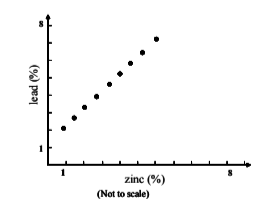
\includegraphics[width=0.4\textwidth]{Screenshot_2025_0813_154158.png} 
\caption{}
    \label{fig:Q1}
    \end{figure}

\hfill(GATE MN 2011)

\begin{enumerate}
 \begin{multicols}{4}
    \item 1.0
    \item 0.7
    \item 0.5
    \item 0
    \end{multicols}
\end{enumerate}

\item The two vectors are orthonormal, if

	\hfill(GATE MN 2011)
	\begin{enumerate}

    \item vector product is zero and norm of each vector is also zero
    \item vector product is one and norm of each vector is also one
    \item cross product is zero and norm of each vector is one
    \item cross product is one and norm of each vector is zero
    
\end{enumerate}

\item The value of 
\[
\lim_{x \to 0} \frac{1}{x} \left( \sqrt{1+x} - \sqrt{1-x} \right) \ \text{is}
\]

\hfill(GATE MN 2011)
\begin{enumerate}
\begin{multicols}{4}
    \item 0
    \item 1
    \item 2
    \item 3
    \end{multicols}
\end{enumerate}

\item The infinite series $1 + \frac{1}{2} + \frac{1}{4} + \frac{1}{8} + \cdots$ is

	\hfill(GATE MN 2011)
\begin{enumerate}
\begin{multicols}{4}
    \item convergent
    \item divergent
    \item oscillatory
    \item semi-convergent
    \end{multicols}
\end{enumerate}

\item The largest area of a rectangular shaft for a given constant perimeter is obtained when length is

	\hfill(GATE MN 2011)

\begin{enumerate}
\begin{multicols}{2}
    \item 2.5 times of breadth
    \item 1.5 times of breadth
    \item 2 times of breadth
    \item equal to breadth
    \end{multicols}
\end{enumerate}

\item A drive shaft of an engine develops torque of $500$ N$\cdot$m. It rotates at a constant speed of $50$ rpm. The power transmitted by the shaft in kW is

	\hfill(GATE MN 2011)
\begin{enumerate}
\begin{multicols}{4}
    \item 1.46
    \item 2.05
    \item 2.62
    \item 4.32
    \end{multicols}
\end{enumerate}

\item A mine winder cage traveling $450$ m from pit bottom to pit top is following a three period duty cycle as shown in the figure below. The maximum velocity attained by the cage in m/s is

\begin{figure}[H]
    \centering
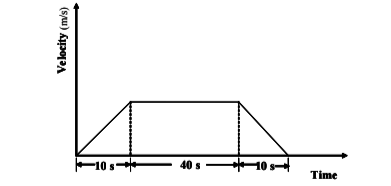
\includegraphics[width=0.5\textwidth]{Screenshot_2025_0813_160511.png} 
\caption{}
    \label{fig:Q7}
    \end{figure}

\hfill(GATE MN 2011)
\begin{enumerate}
		\begin{multicols}{4}
    \item 7.5
    \item 9.0
    \item 11.0
    \item 12.0
	    \end{multicols}
\end{enumerate}

\item Stress concentration at a point on the wall of a vertical shaft results in a compressive stress of $59.66$ MPa. The wall rock mass has an unconfined compressive strength of $89.49$ MPa. The safety factor of the shaft wall at the point is

	\hfill(GATE MN 2011)
\begin{enumerate}
\begin{multicols}{4}
    \item 0.67
    \item 0.86
    \item 1.23
    \item 1.50
	    \end{multicols}
\end{enumerate}

\item A core sample of $54$ mm diameter having Young$’$s modulus of $68.97$ GPa fails in uniaxial compression at $0.1\%$ axial strain. The axial load at failure in kN is

	\hfill(GATE MN 2011)
\begin{enumerate}
		\begin{multicols}{4}
    \item 158.00
    \item 68.97
    \item 58.00
    \item 15.80
	    \end{multicols}
\end{enumerate}

\item The maximum number of coal faces in an underground bord and pillar development district is 13. The number of headings in the district is

	\hfill(GATE MN 2011)
\begin{enumerate}
		\begin{multicols}{4}
    \item 3
    \item 5
    \item 6
    \item 7
	    \end{multicols}
\end{enumerate}

\item The whole circle bearing of the line AB is $116^\circ 20'20''$. If there exists an east declination of $20'$, the true quadrantal bearing of line AB is

	\hfill(GATE MN 2011)
\begin{enumerate}
\begin{multicols}{4}
    \item S$41^\circ 59'40''$E
    \item S$43^\circ 39'40''$E
    \item S$45^\circ 59'40''$W
    \item S$47^\circ 59'40''$W
	    \end{multicols}
\end{enumerate}

\item It is proposed to connect two straights of a road by a simple circular curve. If the maximum speed of the vehicle is 60 km/h and the centrifugal ratio for the road is 1/4, the minimum radius of the curve in m is

	\hfill(GATE MN 2011)
\begin{enumerate}
		\begin{multicols}{4}
    \item 113.26
    \item 98.18
    \item 25.46
    \item 15.50
	    \end{multicols}
\end{enumerate}

\item A centrifugal fan rotating at 500 rpm delivers $70$ m$^3$/s of air. If the speed is reduced to 200 rpm, the quantity of air delivered in m$^3$/s will be

	\hfill(GATE MN 2011)
\begin{enumerate}
		\begin{multicols}{4}
    \item 175
    \item 55
    \item 28
    \item 11
	    \end{multicols}
\end{enumerate}

\item According to mine regulations, the value of the fleet angle $\alpha$, in degree of a drum winder installation lies in the range of

	\hfill(GATE MN 2011)
\begin{enumerate}
		\begin{multicols}{4}
    \item $1.5 < \alpha \leq 2.0$
    \item $0 < \alpha \leq 1.5$
    \item $2.0 < \alpha \leq 2.5$
    \item $2.5 < \alpha \leq 3.0$
	    \end{multicols}
\end{enumerate}

\item Water will not be delivered by a centrifugal pump due to

	\hfill(GATE MN 2011)
\begin{enumerate}
		\begin{multicols}{2}
    \item lack of priming
    \item too low discharge head
    \item wrong direction of rotation
    \item partial obstruction at discharge outlet
	    \end{multicols}
\end{enumerate}

\item Match the following

\begin{table}[H]
    \centering\normalsize
\begin{tabular}{ll}
	\textbf{Mine car type} & \textbf{Mode of unloading} \\
P. Granby & 1. Bottom opening \\
Q. Gable bottom & 2. Both side tilting \\
R. Drop bottom & 3. Single side opening \\
S. Rocker dump & 4. Both side opening
\end{tabular}
\caption{}
    \label{tab:Q16}
\end{table}

\hfill(GATE MN 2011)

\begin{enumerate}
		\begin{multicols}{2}
    \item P-2, Q-4, R-3, S-1
    \item P-4, Q-1, R-3, S-2
    \item P-3, Q-1, R-4, S-2
    \item P-3, Q-4, R-1, S-2
	    \end{multicols}
\end{enumerate}

\item Mean air temperature of a 450 m deep downcast shaft is $29^\circ$C and that of the upcast shaft is $37^\circ$C. The height of the motive column in m is

	\hfill(GATE MN 2011)
\begin{enumerate}
\begin{multicols}{4}
    \item 8.2
    \item 9.5
    \item 11.6
    \item 12.8
	    \end{multicols}
\end{enumerate}

\item The total pressure and the static pressure measured at a point in a ventilation duct are 20 mm and 10 mm of water gauge respectively. If density of air is $1.2\ \text{kg/m}^3$, the velocity of the air in m/s is

	\hfill(GATE MN 2011)
\begin{enumerate}
		\begin{multicols}{4}
    \item 14.08
    \item 12.78
    \item 8.53
    \item 6.24
	    \end{multicols}
\end{enumerate}

\item The type of fire extinguisher that must \textbf{NOT} be used in case of fire in an electric substation located in an underground metal mine is

	\hfill(GATE MN 2011)
\begin{enumerate}
		\begin{multicols}{4}
    \item multi-purpose dry chemical extinguisher
    \item CO$_2$ snow extinguisher
    \item dry chemical powder extinguisher
    \item foam extinguisher
	    \end{multicols}
\end{enumerate}

\item ISO 9000 Quality Systems \textbf{DO NOT} contain

	\hfill(GATE MN 2011)
\begin{enumerate}
		\begin{multicols}{4}
    \item legal provisions
    \item measurement
    \item document control
    \item standardization
	    \end{multicols}
\end{enumerate}

\item Air samples collected from the intake and the return gates of a retreating longwall face show methane concentration values of 0.1\% and 0.8\% respectively. The production from the longwall face is 2000 tonne/day and the air quantity circulating the face is 15 m$^3$/s. The rate of methane emission in m$^3$ per tonne of coal produced is

	\hfill(GATE MN 2011)
\begin{enumerate}
		\begin{multicols}{4}
    \item 11.0
    \item 9.5
    \item 5.5
    \item 4.5
	    \end{multicols}
\end{enumerate}

\item The time study data of an equipment deployed in a mine during a calendar month is given below.\\
Total working hours = 400\\
Total maintenance hours = 100\\
Total hours of actual work = 240\\
The percentage of utilization of the equipment is

\hfill(GATE MN 2011)
\begin{enumerate}
		\begin{multicols}{4}
    \item 85
    \item 80
    \item 65
    \item 60
	    \end{multicols}
\end{enumerate}

\item 
100 ml of waste water is allowed to evaporate in a dish weighing 48.6232 g. The weight of the dish with dry solids is 48.6432 g. The concentration of dry solids in waste water in mg/l is

\hfill(GATE MN 2011)
\begin{enumerate}
		\begin{multicols}{4}
    \item 200
    \item 220
    \item 260
    \item 320
	    \end{multicols}
\end{enumerate}

\item 
A longwall face cut by double back shuffle method can be only worked with 

\hfill(GATE MN 2011)
\begin{enumerate}
		\begin{multicols}{2}
    \item fixed drum shearer
    \item single ended ranging drum shearer
    \item double ended ranging drum shearer
    \item plough
	    \end{multicols}
\end{enumerate}

\item 
Proximate analysis of 50 g of a coal sample shows the following: \\
Moisture = 0.80 g \\
Ash = 7.85 g \\
Volatile matter = 15.90 g \\
The fixed carbon in percentage on a dry, ash free basis is 

\hfill(GATE MN 2011)
\begin{enumerate}
		\begin{multicols}{4}
    \item 83
    \item 66
    \item 55
    \item 45
	    \end{multicols}
\end{enumerate}

\item 
For an oil exploration drilling, chance of striking an oil reservoir is 1 out of 15. If an oil exploration company decides to explore 5 sites, the probability of striking at least one successful oil reservoir is 

\hfill(GATE MN 2011)
\begin{enumerate}
		\begin{multicols}{4}
    \item 0.292
    \item 0.250
    \item 0.034
    \item 0.0024
	    \end{multicols}
\end{enumerate}

\item 
Product of the eigen values of the matrix $A$ is\\ 

$\vec{A} = \myvec{
3 & 2 & 5 \\
2 & 2 & 1 \\
1 & 5 & 4
}$

\hfill(GATE MN 2011)

\begin{enumerate}
		\begin{multicols}{4}
    \item 6
    \item 8
    \item 10
    \item 35
	    \end{multicols}
\end{enumerate}

\item 
For the equation $\frac{dy}{dx} = 2x + 3y$, the value of $y$ at $x = 0.1$ in one step using Runge-Kutta fourth order method for the condition $y = 1$ when $x = 0$, is 

\hfill(GATE MN 2011)
\begin{enumerate}
		\begin{multicols}{4}
    \item 0.3608
    \item 1.2508
    \item 1.3608
    \item 1.4625
	    \end{multicols}
\end{enumerate}

\item 
Value of the integral $\int_{0}^{1} \sqrt{\frac{1+x}{1-x}} \, dx$ is 

\hfill(GATE MN 2011)
\begin{enumerate}
		\begin{multicols}{4}
    \item $\frac{\pi}{2} - 1$
    \item $\frac{\pi}{2} + 1$
    \item $\pi - 1$
    \item $\pi + 1$
	    \end{multicols}
\end{enumerate}

\item A 1 tonne mine car traveling at a constant speed o    f 10 km/h collides with a stationary buffer and co    mes to rest. If the buffer spring stiffness is 200     kN/m, the maximum compression in the spring in mm     is                        

	\hfill(GATE MN 2011)
\begin{enumerate}                                 
	\begin{multicols}{4}                     
	\item 49                                 
	\item 98                                 
	\item 196                                
	\item 247                                
	             \end{multicols}              
\end{enumerate}


\item In an iron ore handling port, a barge is pulled by ropes using two tugboats as shown in the figure. In equilibrium, the resultant of the forces $T_1$ and $T_2$ along the axis of the barge in the direction of its travel is $5000 \, \mathrm{N}$. The tensions $T_1$ and $T_2$ in N respectively are

	\hfill(GATE MN 2011)

\begin{figure}[H]
    \centering
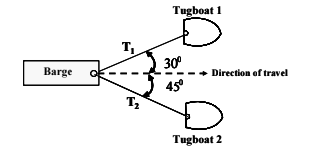
\includegraphics[width=0.4\textwidth]{Screenshot_2025_0813_192351.png}
\caption{}
    \label{fig:Q31}
    \end{figure}

\begin{enumerate}
		\begin{multicols}{2}
    \item 9700 and 6831
    \item 6831 and 9700
    \item 3660 and 2588
    \item 2588 and 3660
	    \end{multicols}
\end{enumerate}

\item A flat belt conveyor is carrying coal of bulk density $1\, \mathrm{tonne/m^3}$ at a rate of $400 \, \mathrm{tonne/h}$. The belt speed is $3\, \mathrm{m/s}$. Coal is spread over the belt covering 80\% of the belt width in a shape of a triangle. If the pile height is $1/4$ of the belt width, the width of the belt in mm is

	\hfill(GATE MN 2011)
\begin{enumerate}
		\begin{multicols}{4}
    \item 1109
    \item 909
    \item 709
    \item 609
	    \end{multicols}
\end{enumerate}

\item Match the following

 \begin{figure}[H]
    \centering
        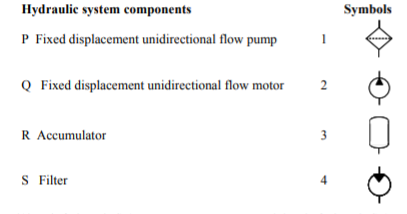
\includegraphics[width=0.7\textwidth]{Screenshot_2025_0816_113416.png}
	    \caption{}
    \label{fig:Q33}
    \end{figure}


    \hfill(GATE MN 2011)
\begin{enumerate}
		\begin{multicols}{2}
    \item P-4, Q-2, R-3, S-1
    \item P-2, Q-4, R-3, S-1
    \item P-3, Q-2, R-1, S-4
    \item P-2, Q-3, R-1, S-4
\end{multicols}
\end{enumerate}

\item Match the following
	\begin{table}[H]
    \centering\normalsize
\begin{tabular}{c c c}                
\textbf{Method of mining} & \textbf{Stope support} & \textbf{Ore loading}  \\   
P. Shrinkage stoping & 1. Insitu pillar & a. Overhead mucker  \\        
Q. Blasthole stoping & 2. Broken ore & b. Pneumatic autoloader \\              
R. Top slicing & 3. Timber mat & c. Load haul dumper  \\                
\end{tabular}
\caption{}
    \label{tab:Q32}
\end{table}

\hfill(GATE MN 2011)
\begin{enumerate}
		\begin{multicols}{2}
    \item P-2-a, Q-1-c, R-3-b
    \item P-2-a, Q-3-c, R-1-b
    \item P-2-b, Q-3-c, R-1-a
    \item P-3-c, Q-2-a, R-1-b
	    \end{multicols}
\end{enumerate}

\item A typical case of gravity loading under complete lateral restraint in flat strata is shown in the figure below. The physico-mechanical parameters of the strata are given in the table. The in situ stresses $(\sigma_Z, \sigma_H)$ on the top of the coal seam in MPa are:


\begin{figure}[H]
    \centering
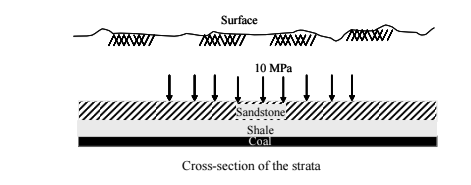
\includegraphics[width=0.6\textwidth]{Screenshot_2025_0813_193403.png} 
\caption{}
    \label{fig:Q35}
    \end{figure}
\begin{table}[H]
\centering
	\small
\begin{tabular}{|c|c|c|c|c|}
\hline
\textbf{Strata} & \textbf{Thickness (m)} & \textbf{Specific Gravity} & \textbf{Young's  Modulus (GPa)} & \textbf{Shear Modulus (GPa)} \\
\hline
Sandstone & 50 & 2.35 & 26.40 & 12.50 \\
\hline
Shale & 25 & 2.15 & 20.50 & 8.25 \\
\hline
Coal & 20 & 1.52 & 2.41 & 0.95 \\
\hline

\end{tabular}
\caption{}
    \label{tab:Q35}


	\hfill(GATE MN 2011)

\end{table}
\begin{enumerate}
\begin{multicols}{4}
    \item $(10.17, 2.54)$
    \item $(10.17, 3.69)$
    \item $(11.68, 3.69)$
    \item $(11.68, 2.54)$
	    \end{multicols}
\end{enumerate}



\item The sale value of chromite ore from an open pit mine is Rs.\ 6500 per tonne. 
Cost of mining, excluding stripping cost, is Rs.\ 2450 per tonne. 
If the cost of stripping is Rs.\ 1150 per m$^3$, the breakeven stripping ratio in m$^3$/tonne is

\hfill(GATE MN 2011)
\begin{multicols}{4}
\begin{enumerate}
  \item 2.18
  \item 3.52
  \item 3.65
  \item 4.25
\end{enumerate}
\end{multicols}

\item An investment at 10\% yearly interest rate, compounded quarterly, accumulates to a sum of Rs.\ 120,000 in 5 years. 
The present value of the sum in rupees is

\hfill(GATE MN 2011)
\begin{multicols}{4}
\begin{enumerate}
  \item 72,233
  \item 74,511
  \item 88,232
  \item 106,063
\end{enumerate}
\end{multicols}

\item A toxic gas flows into a mine working place at the rate of 2.52 m$^3$/min. 
The concentration of the gas in the intake air is 0.25\%. 
The minimum quantity of intake air in m$^3$/min required to dilute the gas to its threshold limit value of 1.0\% is

\hfill(GATE MN 2011)
\begin{multicols}{4}
\begin{enumerate}
  \item 123
  \item 252
  \item 295
  \item 333
\end{enumerate}
\end{multicols}

\item An exhaust fan attached to an evasee of 18 m$^2$ cross-sectional area at the outlet circulates 150 m$^3$/s of air at the pressure of 1000 Pa in a mine ventilation system. 
The ratio of the inlet to outlet area of the evasee is 1:4 and the density of air is 1.2 kg/m$^3$. 
The quantity of air circulated in the mine in absence of evasee is 120 m$^3$/s. 
The evasee efficiency in \% is

\hfill(GATE MN 2011)
\begin{multicols}{4}
\begin{enumerate}
  \item 57.6
  \item 43.2
  \item 39.06
  \item 37.7
\end{enumerate}
\end{multicols}

\item A fan circulates 24 m$^3$/s of air at a pressure of 1200 Pa in a ventilation district. 
It is intended to reduce the air quantity to 16 m$^3$/s by placing a regulator. 
Assuming the pressure remains unchanged, the size of the regulator in m$^2$ is

\hfill(GATE MN 2011)
\begin{multicols}{4}
\begin{enumerate}
  \item 1.48
  \item 0.74
  \item 0.37
  \item 0.18
\end{enumerate}
\end{multicols}

\item An air sample taken from the return airway of a district contains the following gases. 
The Graham’s ratio for the district is

\begin{table}[H]
    \centering\normalsize
\begin{tabular}{|c|c|}
\hline
Gas & Concentration (\%) \\ \hline
CO$_2$ & 0.40 \\ \hline
H$_2$ & 1.17 \\ \hline
O$_2$ & 19.92 \\ \hline
N$_2$ & 78.49 \\ \hline
CO & 0.02 \\ \hline
\end{tabular}

\caption{}
    \label{tab:Q41}
\end{table}


\hfill(GATE MN 2011)
\begin{multicols}{4}
\begin{enumerate}
  \item 5.6
  \item 4.8
  \item 3.0
  \item 2.3
\end{enumerate}
\end{multicols}

\item An incandescent headlight of a mining vehicle is of spot beam type with a beam angle of 30$^\circ$. 
The spherical surface in m$^2$ subtended by the lighted beam at a distance of 5 m from the headlight is

\hfill(GATE MN 2011)
\begin{multicols}{4}
\begin{enumerate}
  \item 7.5
  \item 15
  \item 21
  \item 25
\end{enumerate}
\end{multicols}

\item The thickness of a coal deposit is represented by a spherical semi-variogram model with sill of 5 m$^2$. 
If the semi-variogram value at lag distance $h$ is 3 m$^2$, the correlogram value at the same lag distance is

\hfill(GATE MN 2011)
\begin{multicols}{4}
\begin{enumerate}
  \item 0.4
  \item 2.0
  \item 2.5
  \item 5.0
\end{enumerate}
\end{multicols}

\item The total cost $C$ (lakh rupees) of a longwall face of length $L$ in m is given by the equation
\[
C = 0.1L + \frac{1562.5}{L} + 300
\]
Length of the face in m for the minimum total cost is

\hfill(GATE MN 2011)
\begin{multicols}{4}
\begin{enumerate}
  \item 40
  \item 125
  \item 156
  \item 300
\end{enumerate}
\end{multicols}

\item 20 plain detonators in series, each of 2$\Omega$ resistance, are fired by a DC exploder supplying a current of 1.25 A. 
If 250 mJ energy is spent to fire the detonators, the time required in millisecond after detonator initiation is

\hfill(GATE MN 2011)
\begin{multicols}{4}
\begin{enumerate}
  \item 4
  \item 8
  \item 12
  \item 16
\end{enumerate}
\end{multicols}


\item A sudden increase of CO incidence has occurred in an underground mine section. A man at point A starts to run out to the main intake of the mine where he will be safe. Refer figure below for the mine section and the logic diagram. The probabilities that he will successfully cross the gallery sections A, B, C, D, E, and F are 0.9, 0.8, 0.7, 0.8, 0.7 and 0.9 respectively. The probability that he will successfully reach the main intake is  

    
\begin{center}
\begin{minipage}{0.45\textwidth}

\centering
\begin{figure}[H]
    \centering
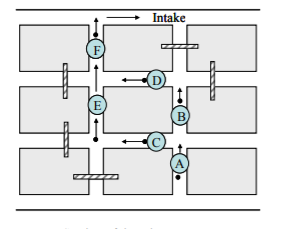
\includegraphics[width=\textwidth]{Screenshot_2025_0816_114426.png} \\ 
\caption{}
    \label{fig:Q4}
    \end{figure}
\textit{Section of the mine}
\end{minipage}
\hfill
\begin{minipage}{0.45\textwidth}
\centering
\begin{figure}[H]
    \centering
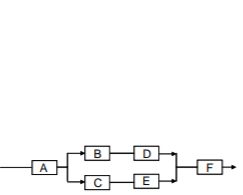
\includegraphics[width=\textwidth]{Screenshot_2025_0816_114537.png} \\ 
\caption{}
    \label{fig:Q4}
    \end{figure}
\textit{Series-parallel logic diagram}
\end{minipage}
\end{center}


\hfill(GATE MN 2011)

\begin{multicols}{4}
\begin{enumerate}
\item 0.40  
\item 0.51  
\item 0.66  
\item 0.77  
\end{enumerate}
\end{multicols}

\item In an underground correlation survey by the Weisbach triangle (figure below) the following data are obtained:  
\begin{figure}[H]
    \centering
        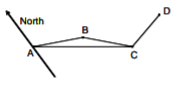
\includegraphics[width=0.7\textwidth]{Screenshot_2025_0816_112932.png}
	    \caption{}
    \label{fig:Q47}
    \end{figure} 


    \hfill(GATE MN 2011)
\begin{multicols}{2}
\begin{enumerate}
\item $102^\circ 27' 16''$  
\item $114^\circ 41' 49''$  
\item $115^\circ 27' 16''$  
\item $179^\circ 14' 16''$
\end{enumerate}
\end{multicols}

\textbf{Common Data Questions}

\textbf{Common Data for Questions 48 and 49:}\\  
A concentrator pilot plant is fed with 1 tonne of copper ore at ROM grade of 1.5\% Cu. Metal recovery in the concentrator pilot plant is 90\% and the grade of copper in concentrate is 20\%.  

\item The amount of copper in concentrate in kg is:  

	\hfill(GATE MN 2011)

\begin{multicols}{4}
\begin{enumerate}
\item 13.5  
\item 14.0  
\item 14.5  
\item 15.0  
\end{enumerate}
\end{multicols}

\item Amount of concentrate produced from 1 tonne of ore in kg is: 

	\hfill(GATE MN 2011)

\begin{multicols}{4}
\begin{enumerate}
\item 75.0  
\item 72.0  
\item 70.0  
\item 67.5  
\end{enumerate}
\end{multicols}

\textbf{Common Data for Questions 50 and 51:} A mine ventilation system consists of two splits A and B with resistances of $0.8 \, \text{Ns}^2/\text{m}^8$ respectively as shown in figure. Trunk airways have resistance of $0.2 \, \text{Ns}^2/\text{m}^8$. The main fan generating pressure of 500 Pa.

    \begin{figure}[H]
    \centering
        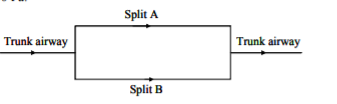
\includegraphics[width=0.7\textwidth]{Screenshot_2025_0816_115916.png}
	    \caption{}
    \label{fig:Q50}
    \end{figure}

\item The air quantities in m$^3$/s circulated in the splits A and B respectively are:  

	\hfill(GATE MN 2011)

\begin{multicols}{4}
\begin{enumerate}
\item 20 and 30  
\item 30 and 20  
\item 20 and 10  
\item 40 and 10  
\end{enumerate}
\end{multicols}

\item The flows in the two splits are equalized by placing a booster fan in split B. Assume that the fan pressure does not change after installation of the booster fan. The size of the booster fan in Pa is:  

	\hfill(GATE MN 2011)

\begin{multicols}{4}
\begin{enumerate}
\item 749.05  
\item 850.08  
\item 950.02  
\item 1000.50  
\end{enumerate}
\end{multicols}


\textbf{Linked Answer Questions}


\textbf{Statement for Linked Answer Questions 52 and 53:}\\
A 400 V, 3 phase, star connected induction motor takes a line current of 10 A with 0.86 p.f. lagging. Total stator losses are 5\% of the input. Rotor copper losses are 4\% of the input to the rotor, and mechanical losses are 3\% of the input to the rotor.



\item The input power to the rotor in Watts is

	\hfill(GATE MN 2011)
\begin{multicols}{4}
\begin{enumerate}
\item 5958  
\item 5788  
\item 5660  
\item 5532  
\end{enumerate}
\end{multicols}

\item The shaft output power in Watts is

	\hfill(GATE MN 2011)
\begin{multicols}{4}
\begin{enumerate}
\item 5562  
\item 5490  
\item 5434  
\item 5264  
\end{enumerate}
\end{multicols}



\textbf{Statement for Linked Answer Questions 54 and 55:}\\
The bolts are spaced at 1.5 m centre-to-centre in a square pattern as shown in the figure below. The tensile stress in 22 mm diameter bolt rod is 193.35 MPa. The unit weight of the roof layer is 25 kN/m$^{3}$.

\begin{center}
Plan view of rock bolting pattern (figure)
\begin{figure}[H]
    \centering
        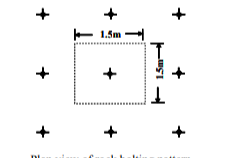
\includegraphics[width=0.7\textwidth]{Screenshot_2025_0816_120814.png}
	    \caption{}
    \label{fig:Q54}
    \end{figure}
\end{center}

\item The axial load in the bolt rod in kN is

	\hfill(GATE MN 2011)
\begin{multicols}{4}
\begin{enumerate}
\item 294.0  
\item 173.5  
\item 147.0  
\item 73.5  
\end{enumerate}
\end{multicols}

\item At equilibrium, the thickness of the roof layer supported by the bolt in m is

	\hfill(GATE MN 2011)
\begin{multicols}{4}
\begin{enumerate}
\item 1.31  
\item 2.4  
\item 2.62  
\item 3.08  
\end{enumerate}
\end{multicols}



\textbf{General Aptitude (GA) Questions}

\noindent
\textbf{Q.56 -- Q.60 carry one mark each.}



\item Choose the word from the options given below that is most nearly opposite in meaning to the given word: \\
\textbf{Deference}

\hfill(GATE MN 2011)

\begin{enumerate}
\item aversion  
\item resignation  
\item suspicion  
\item contempt  
\end{enumerate}


\item Choose the most appropriate word(s) from the options given below to complete the sentence. \\
\textbf{We lost confidence in him because he never \underline{\hspace{2cm}} the grandiose promises he had made.}


\hfill(GATE MN 2011)
\begin{enumerate}
\item delivered  
\item deliberated on  
\item forgot  
\item reneged on  
\end{enumerate}

\item Choose the word or phrase that best completes the sentence below. \\
\textbf{\underline{\hspace{2cm}} in the frozen wastes of Arctic takes special equipment.}


\hfill(GATE MN 2011)
\begin{enumerate}
\item To survive  
\item Surviving  
\item Survival  
\item That survival  
\end{enumerate}

\item In how many ways 3 scholarships can be awarded to 4 applicants, when each applicant can receive any number of scholarships?


	\hfill(GATE MN 2011)
\begin{multicols}{4}
\begin{enumerate}
\item 4
\item 12
\item 64
\item 81
\end{enumerate}
\end{multicols}

\item Choose the most appropriate word from the options given below to complete the following sentence.  

\textit{The \underline{\hspace{2cm}} of evidence was on the side of the plaintiff since all but one witness testified that his story was correct.}


\hfill(GATE MN 2011)
\begin{enumerate}
\item paucity
\item propensity
\item preponderance
\item accuracy
\end{enumerate}


\textbf{Q.61 to Q.65 carry two marks each.}



\item If $(2y+1)(y+2) < 1$, then which of the following alternatives gives the \textbf{CORRECT} range of $y$?

	\hfill(GATE MN 2011)

\begin{multicols}{4}
\begin{enumerate}
\item $-2 < y < 2$
\item $-2 < y < 1$
\item $-3 < y < 1$
\item $-4 < y < 1$
\end{enumerate}
\end{multicols}

\item A student attempted to solve a quadratic equation in $x$ twice. However, in the first attempt, he incorrectly wrote the constant term and ended up with the roots as (4,3). In the second attempt, he incorrectly wrote down the coefficient of $x$ and got the roots as (3,2). Based on the above information, the roots of the correct quadratic equation are  

	\hfill(GATE MN 2011)

\begin{multicols}{4}
\begin{enumerate}
\item (3,4)
\item (3,-4)
\item (6,1)
\item (4,2)
\end{enumerate}
\end{multicols}

\item L, M and N are waiting in a queue meant for children to enter the zoo. There are 5 children between L and M, and 8 children between M and N. If there are 3 children ahead of N and 21 children behind L, then what is the minimum number of children in the queue?  


	\hfill(GATE MN 2011)
\begin{multicols}{4}
\begin{enumerate}
\item 28
\item 27
\item 41
\item 40
\end{enumerate}
\end{multicols}

\item Four archers P, Q, R and S try to hit a bull’s eye during a tournament consisting of seven rounds. As illustrated in the figure below, a player receives 10 points for hitting the bull’s eye, 5 points for hitting within the inner circle and 1 point for hitting within the outer circle.  
	\begin{figure}[H]
    \centering
        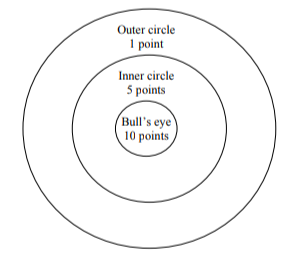
\includegraphics[width=0.7\textwidth]{Screenshot_2025_0816_123811.png}
	    \caption{}
    \label{fig:Q64}
    \end{figure}

The final scores received by the players during the tournament are listed in the table below.
\begin{table}[H]
    \centering\normalsize	
\begin{tabular}{|c|c|c|c|c|}
\hline
Round & P & Q & R & S \\
\hline
1 & 1 & 5 & 1 & 10 \\\hline
2 & 10 & 10 & 5 & 1 \\\hline
3 & 1 & 10 & 1 & 5 \\\hline
4 & 10 & 1 & 5 & 1 \\\hline
5 & 1 & 10 & 1 & 5 \\\hline
6 & 10 & 5 & 1 & 1 \\\hline
7 & 5 & 10 & 5 & 1 \\
\hline
\end{tabular}
\caption{}
    \label{tab:Q64}
\end{table}

\bigskip
The most accurate and the most consistent players during the tournament are respectively  

\hfill(GATE MN 2011)
\begin{multicols}{4}
\begin{enumerate}
\item P and S
\item Q and R
\item Q and Q
\item R and Q
\end{enumerate}
\end{multicols}

\item Nimbus clouds are dark and ragged, stratus clouds appear dull in colour and cover the entire sky. Cirrus clouds are thin and delicate, whereas cumulus clouds look like cotton balls.  

It can be inferred from the passage that  

\hfill(GATE MN 2011)
\begin{enumerate}
\item A cumulus cloud on the ground is called fog
\item It is easy to predict the weather by studying clouds
\item Clouds are generally of very different shapes, sizes and mass
\item There are four basic cloud types: stratus, nimbus, cumulus and cirrus
\end{enumerate}

\end{enumerate}

\bigskip
\begin{center}
\textbf{END OF THE QUESTION PAPER}
\end{center}

\end{document}




\end{enumerate}

\end{document}

